\documentclass[svgnames]{beamer}
%\documentclass[svgnames, handout]{beamer}

\usetheme{i4}

\setbeamertemplate{navigation symbols}{}

\usepackage{setspace}
\usepackage{graphicx}
\usepackage{color}
\usepackage{subfigure}
\usepackage{listings}
\usepackage{amsmath}
\usepackage{amssymb}

\usepackage{textpos}

\usepackage{rotating}
\usepackage{xcolor}
\usepackage{colortbl}

\usepackage{gnuplottex}

\usepackage{gnuplot-lua-tikz}
\definecolor{i4red}{rgb}{0.69,0.11,0.18}
\definecolor{i4blue}{rgb}{0.0,0.4,0.62}
\definecolor{i4green}{rgb}{0.0,0.62,0.4}
\definecolor{i4gray}{rgb}{0.827,0.827,0.827}
\definecolor{darkred}{rgb}{0.8,0,0}
\definecolor{myblue}{rgb}{0,0.1,0.6}
\definecolor{myheadblue}{rgb}{0,0.2,0.7}
\definecolor{myred}{rgb}{0.63,.16,.16}
\definecolor{lstshade}{gray}{0.95}
\definecolor{lstframe}{gray}{0.80}
\definecolor{lstcomment}{gray}{0.5}
\definecolor{lstattrib}{rgb}{0,0.34,0}
\definecolor{remark}{rgb}{1.0, 0.9, 0.9}
\definecolor{remarkframe}{rgb}{1.0, 0.7, 0.7}
\definecolor{i4red}{rgb}{0.69,0.11,0.18}
\definecolor{color_c}{rgb}{0.1686,0.5373,0.8431}
\colorlet{lavender}{blue!60!black!20}
\colorlet{darklavender}{blue!60!black!60}
\colorlet{beige}{yellow!70!black!50!white}
\colorlet{c1blue}{color_c!70!white}

%\setlength{\tabcolsep}{8pt}
%\renewcommand{\arraystretch}{1.5}
%
%\setbeamertemplate{section in toc}{%
%    \color{i4red} $\bullet$  \color{i4blue} \inserttocsection \par}
%
%\setbeamertemplate{subsection in toc}{
%    \color{i4red} \quad $\hookrightarrow$ \color{i4blue} \inserttocsubsection \par}


\institute{Friedrich-Alexander Universit\"at Erlangen-N\"urnberg}
\title[Vergleich nichtblockierender Queues]{Praktikum angewandte Systemsoftwaretechnik: \\
Vergleich nichtblockierender Queues} 

\author{Michael Banken \and Lorenz Haspel} % Your name

\date{20.9.2013} % Date, can be changed to a custom date


\begin{document}


\begin{frame}

	\titlepage
\end{frame}

%-----------------------------------------
\begin{frame}
\frametitle{Projekt\"ubersicht}
\begin{itemize}
\item im Rahmen von LAOS/OctoPOS
\item Queues als zentrale Datenstrukur f\"ur die Verwaltung von Threads
\item paralleler Zugriff auf gemeinsame Daten
\item unsere Zielsetzung: Performanzanalyse und die Entwicklung
paralleler Tests mit verschiedenen nichtblockierenden Queues
\end{itemize}
\end{frame}

%-----------------------------------------
\begin{frame}
\frametitle{Durchgef\"uhrte Tests: "Roundtest"}
\begin {figure}
      \begin{center}
	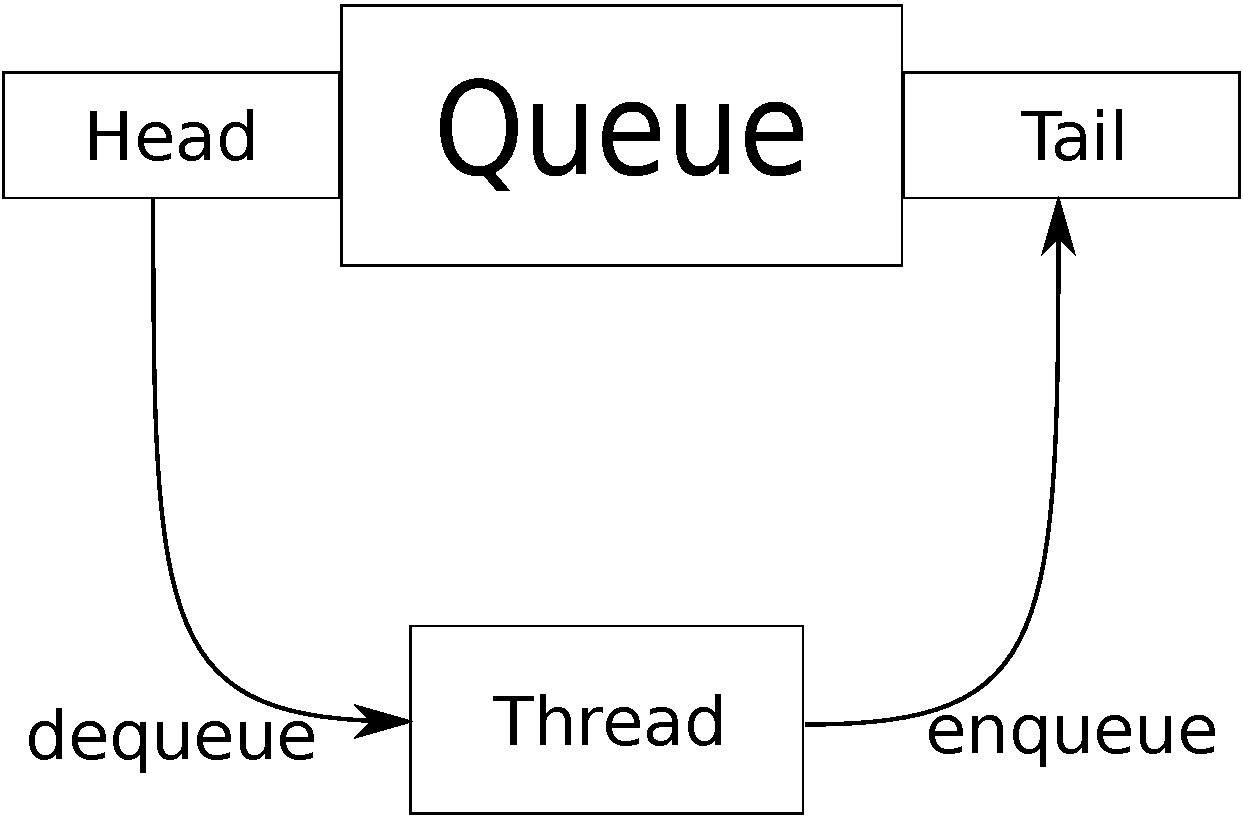
\includegraphics[scale=0.25]{round.pdf}
     \end{center}
\end {figure}

\begin{itemize}
 \item eine Queue, zu Beginn gef\"ullt
 \item Threads entfernen je ein Element aus der Queue und f\"ugen dieses wieder ein.
 \item Elemente bleiben konstant, werden immer wieder verwendet
\end{itemize}
\end{frame}
%-----------------------------------------
\begin{frame}
\frametitle{Durchgef\"uhrte Tests: "Roundtest"}
\begin{itemize}
 \item Versuchsreihen mit variierender Anzahl an Threads und Elementen
 \item feste Gesamtzahl an Operationen
 \item Zeit wird gemessen
 \item drei Testreihen:
\begin{itemize}
 \item halb so viele Elemente wie Threads
 \item genau so viele Elemente wie Threads
 \item doppelt so viele Elemente wie Threads
\end{itemize}
\end{itemize}
\end{frame}

%-----------------------------------------
\begin{frame}
\frametitle{Durchgef\"uhrte Tests: "MPMC-Test"}
\begin {figure}
      \begin{center}
	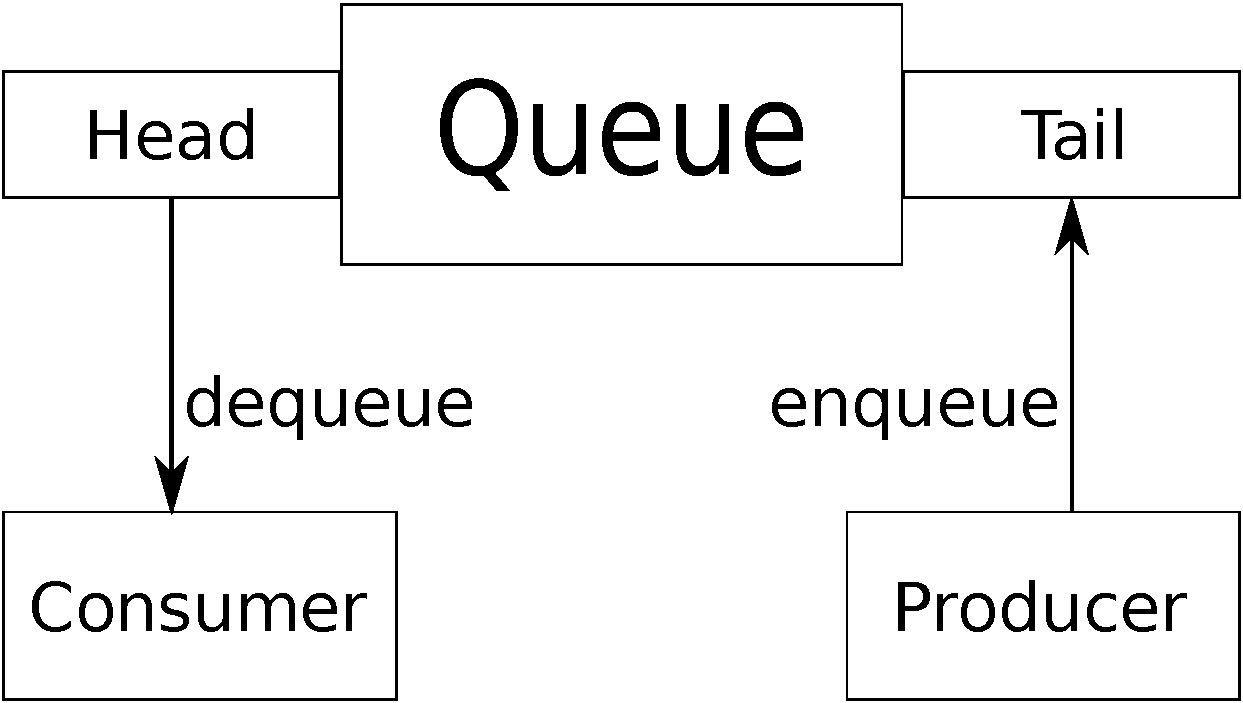
\includegraphics[scale=0.25]{mpmc.pdf}
     \end{center}
\end {figure}

\begin{itemize}
 \item Multiple Producers Multiple Consumers
 \item Queue zu Beginn leer
 \item Produzententhreads f\"ugen Elemente ein
 \item Konsumententhreads nehmen Elemente raus
 \item jedes Element wird nur einmal verwendet


\end{itemize}
\end{frame}

%-----------------------------------------
\begin{frame}
\frametitle{Durchgef\"uhrte Tests: "MPMC-Test"}
\begin{itemize}
 \item Versuchsreihe mit variierender Anzahl an Threads
 \item feste Anzahl an Elementen, die die Queue durchlaufen
 \item zwei Testreihen:
\begin{itemize}
 \item variable Zahl an Produzenten, ein Konsument
 \item gleiche Zahl von Produzenten wie Konsumenten
\end{itemize}


\end{itemize}
\end{frame}

%-----------------------------------------
\begin{frame}
\frametitle{Verwendete Architekturen}
\begin{itemize}
 \item Core i7 aus der Manlobbi:
\begin{itemize}
 \item 4 Kerne, 8 durch Hyperthreading
 \item Tests neben normaler Betriebslast (Programme andere User, X-Server, Ubuntu-Hintergrundprogramme)
\end{itemize}
 \item Haswellrechner "Fastbox":
\begin{itemize}
 \item 8 Kerne, Intel-Haswell Prozessoren
 \item Test von Queues mit naiver Implementierung von Haswell-Transaktionen
 \item atomare Transaktionen auf Prozessorebene
\end{itemize}
 \item 48-Kern-Rechner "Bigbox":
\begin{itemize}
 \item Tests bei massiv parallelem Zugriff
\end{itemize}
\end{itemize}
\end{frame}

%-----------------------------------------
\begin{frame}
\frametitle{Verwendete Queues}
\begin{itemize}
 \item SimpleQueue: Queue mit einem globalen Lock f\"ur en- und dequeue-Operationen
\begin{itemize}
 \item Varianten: Spinlock, Mutex, Haswell-Transaktion
\end{itemize}
 \item TwoLockQueue: Queue mit zwei Locks, je eines f\"ur en- und dequeue Operationen
\begin{itemize}
 \item Varianten: Spinlock, Mutex, Haswell-Transaktionen
\end{itemize}
 \item Michael-Scott-Queue: nicht-blockierende Queue
\begin{itemize}
 \item verwendet CAS-Operationen
\end{itemize}
 \item MPSC-Queue: Multiple-Producers-Single-Consumer-Queue
\begin{itemize}
\item spezialisierte nicht-blockierende Queue
\end{itemize}
\end{itemize}
\end{frame}

%-----------------------------------------

\begin{frame}
\frametitle{Ergebnisse}
\begin {figure}
      \begin{center}
	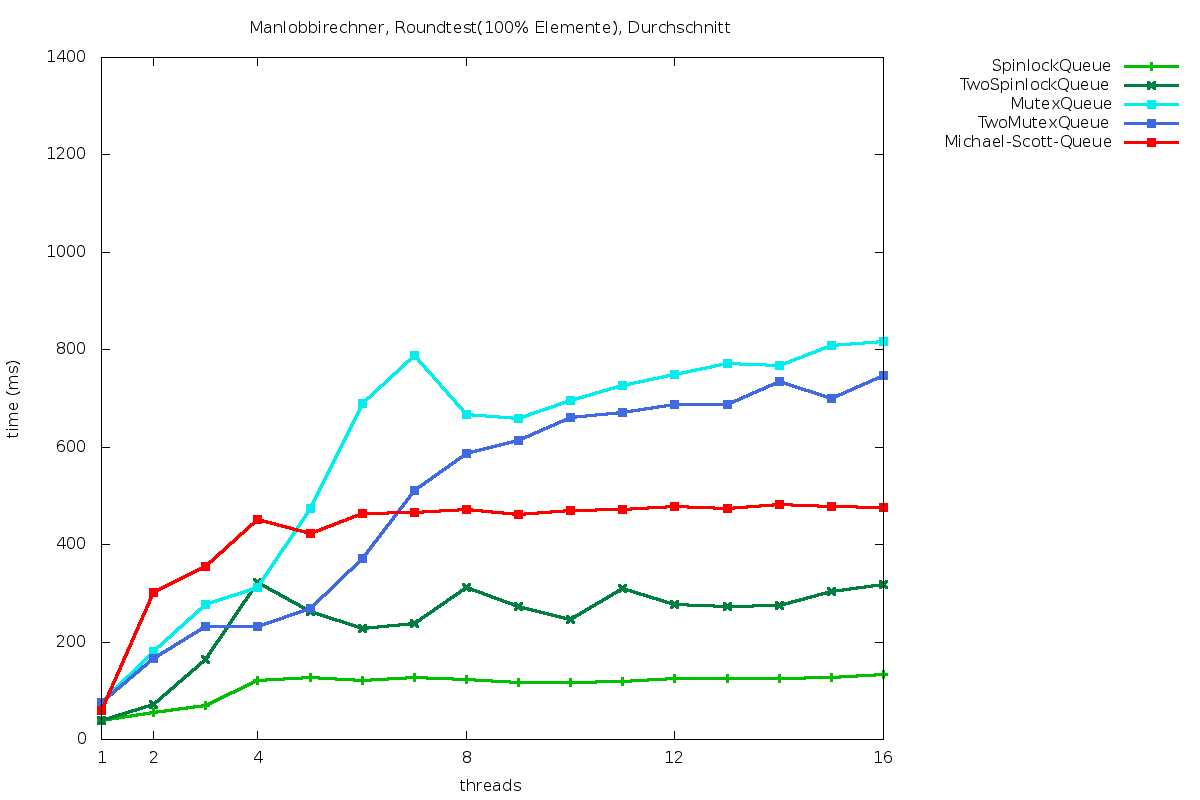
\includegraphics[width=\textwidth]{manr2a.png}
     \end{center}
\end {figure}
\end{frame}

\begin{frame}
\frametitle{Ergebnisse}
\begin {figure}
      \begin{center}
	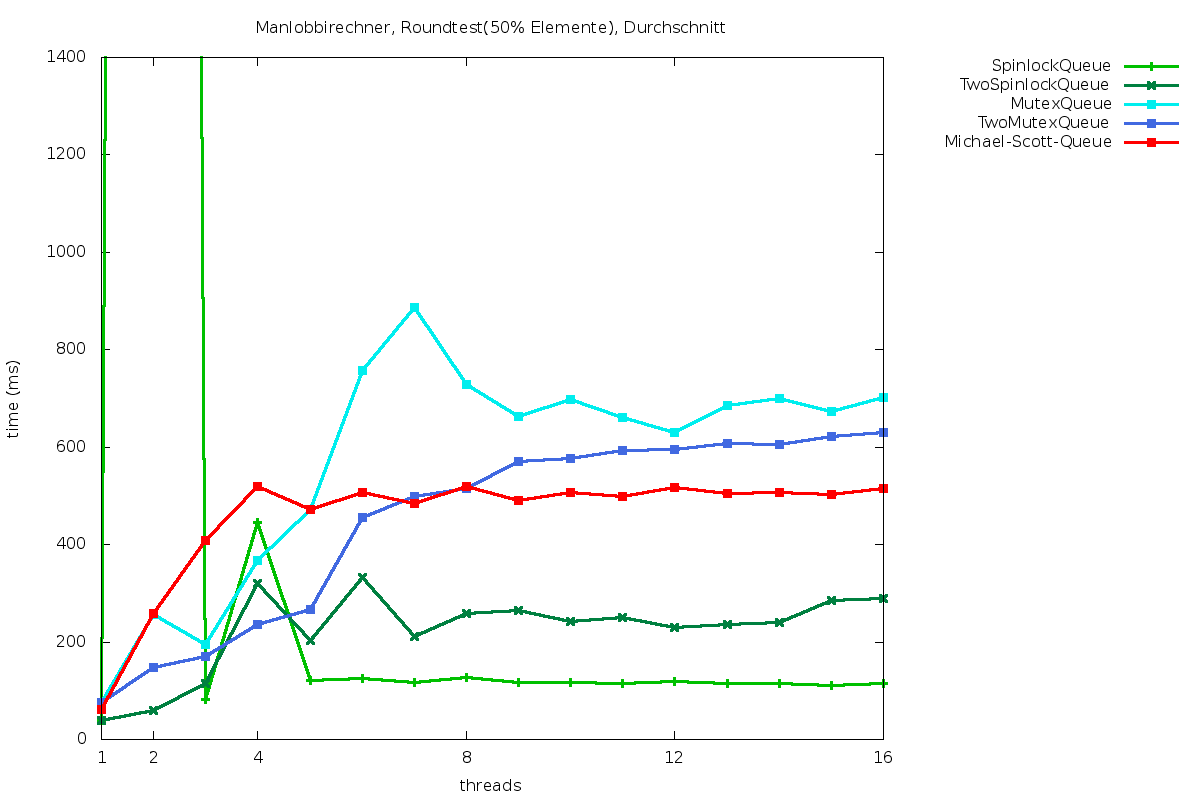
\includegraphics[width=\textwidth]{manr1a.png}
     \end{center}
\end {figure}
\end{frame}
%-----------------------------------------

\begin{frame}
\frametitle{Ergebnisse}
\begin {figure}
      \begin{center}
	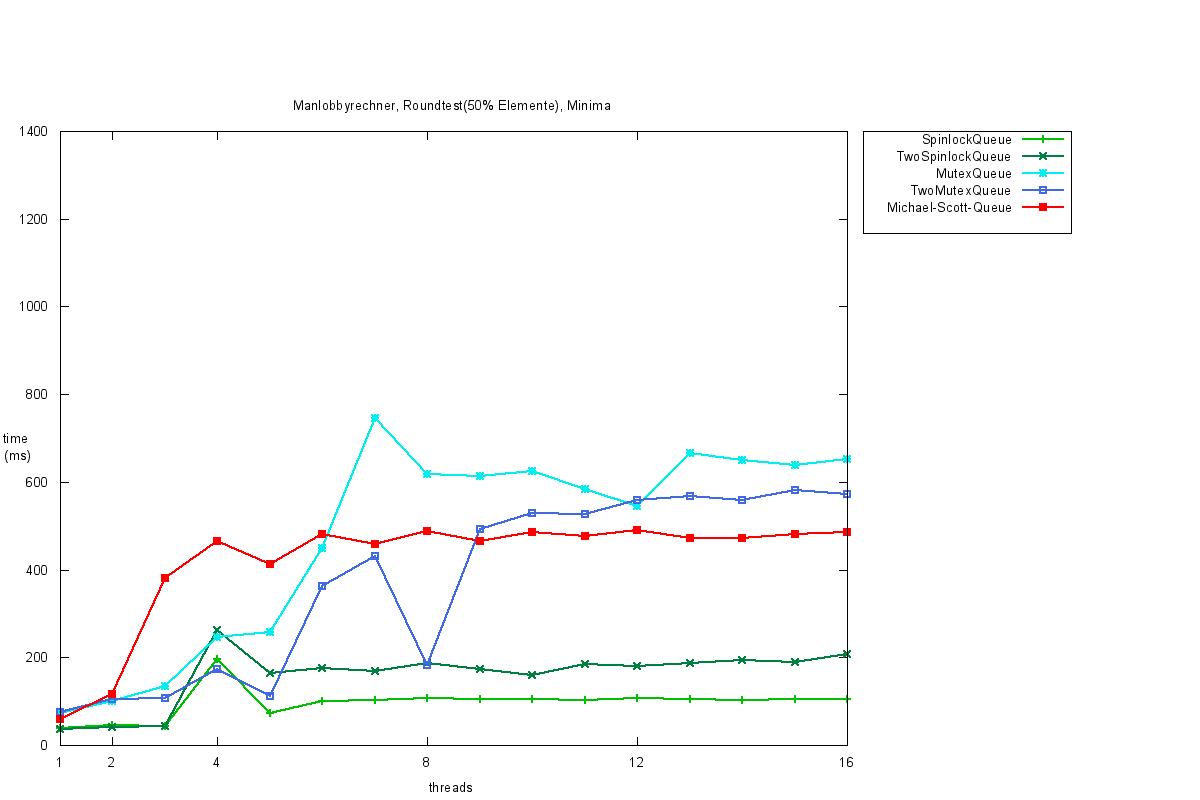
\includegraphics[width=\textwidth]{manr1m.png}
     \end{center}
\end {figure}
\end{frame}

%-----------------------------------------

\begin{frame}
\frametitle{Ergebnisse}
\begin {figure}
      \begin{center}
	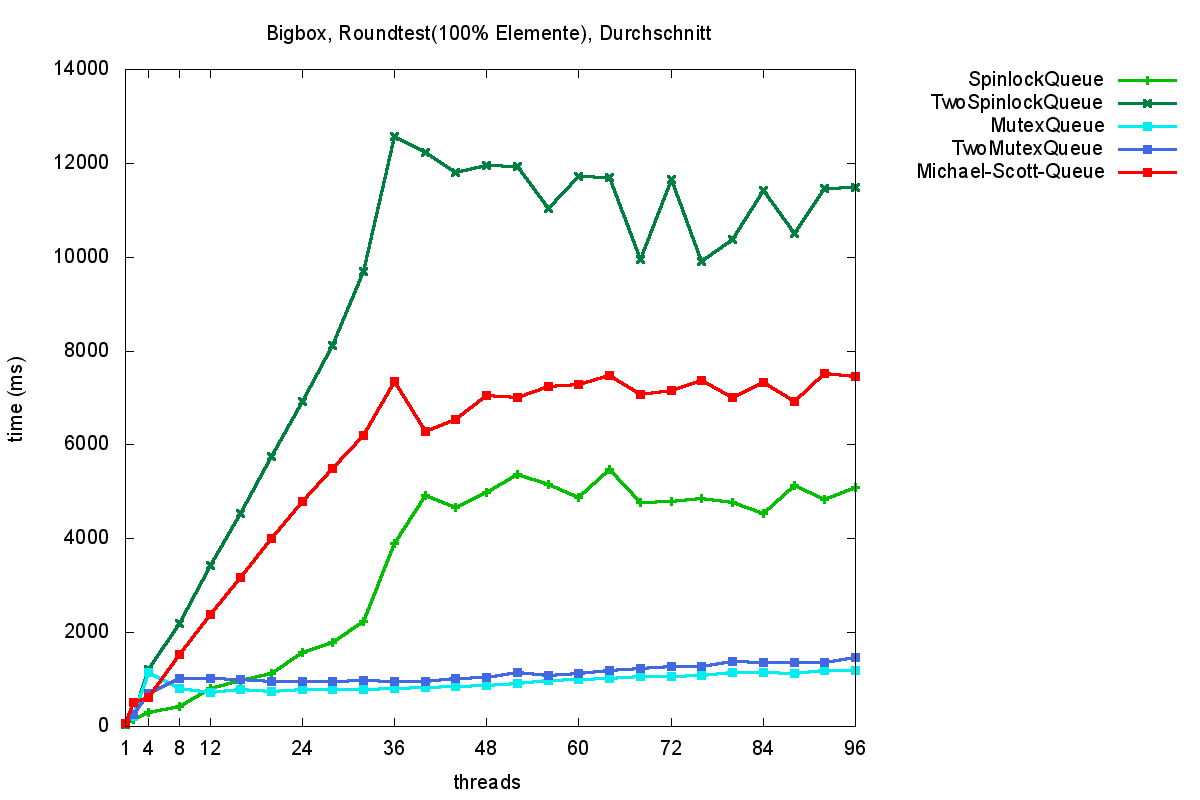
\includegraphics[width=\textwidth]{bigboxr2a.png}
     \end{center}
\end {figure}
\end{frame}
%-----------------------------------------

\begin{frame}
\frametitle{Ergebnisse}
\begin {figure}
      \begin{center}
	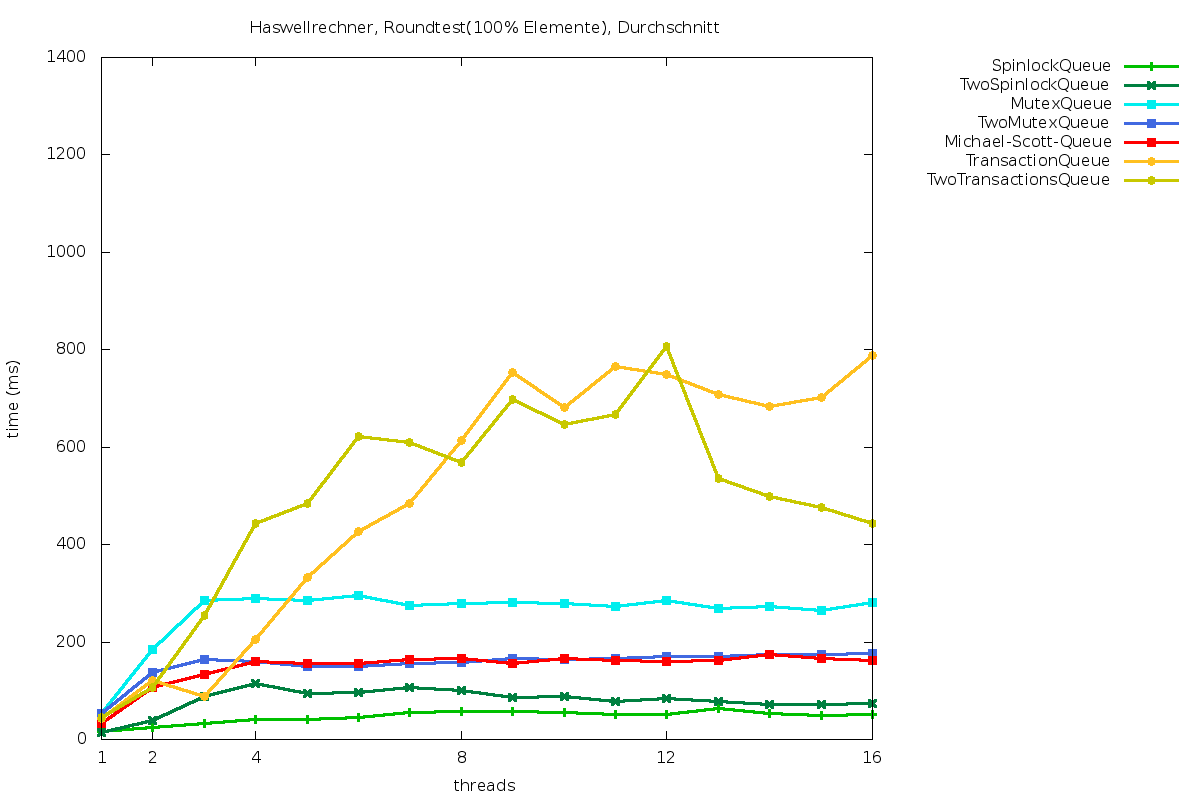
\includegraphics[width=\textwidth]{fastboxr2a.png}
     \end{center}
\end {figure}
\end{frame}

%-----------------------------------------
\begin{frame}
\frametitle{Ergebnisse}
\begin {figure}
      \begin{center}
	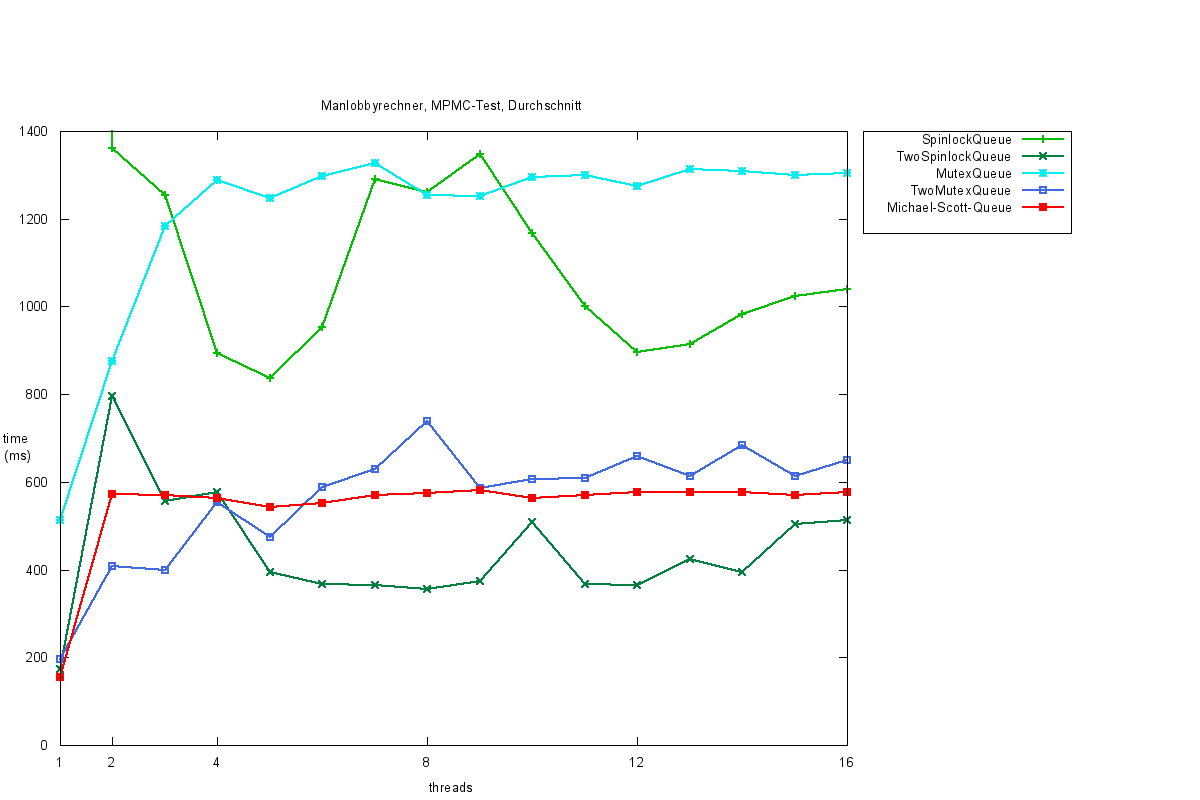
\includegraphics[width=\textwidth]{manma.png}
     \end{center}
\end {figure}
\end{frame}

\begin{frame}
\frametitle{Ergebnisse}
\begin {figure}
      \begin{center}
	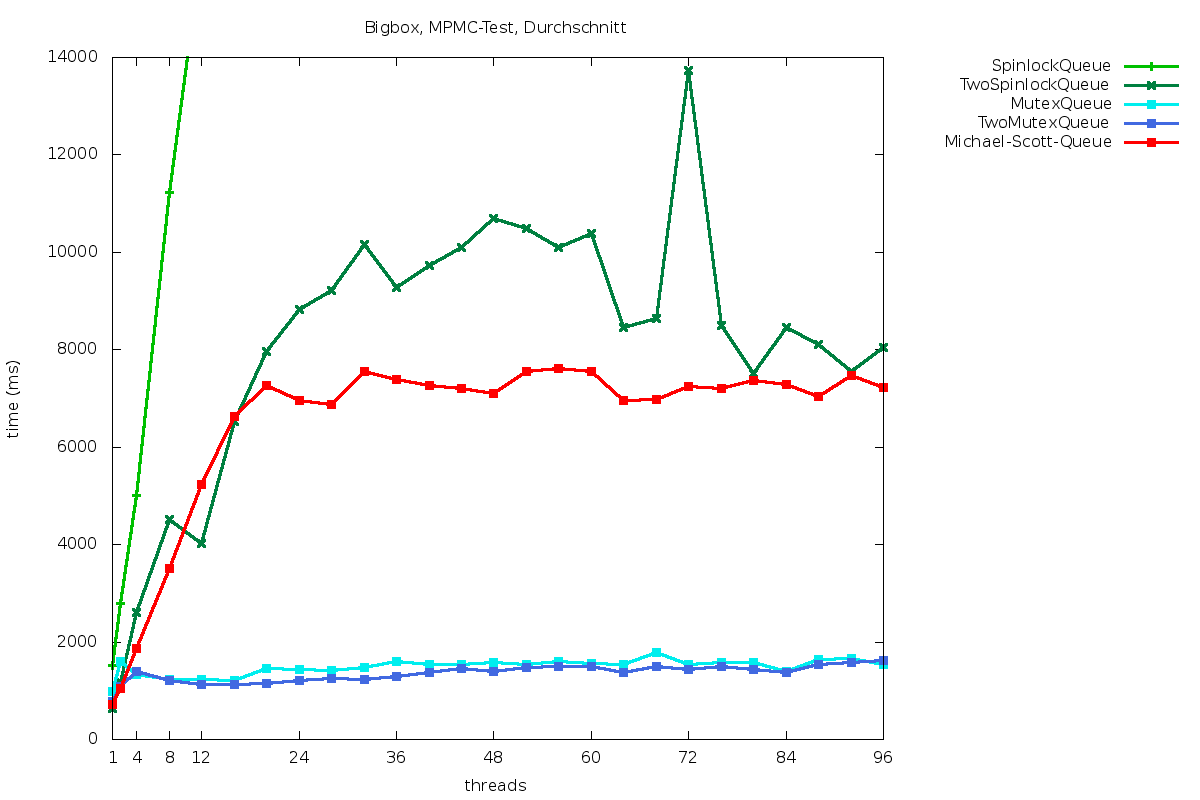
\includegraphics[width=\textwidth]{bigboxma.png}
     \end{center}
\end {figure}
\end{frame}

%-----------------------------------------
\begin{frame}
\frametitle{Ergebnisse}
\begin {figure}
      \begin{center}
	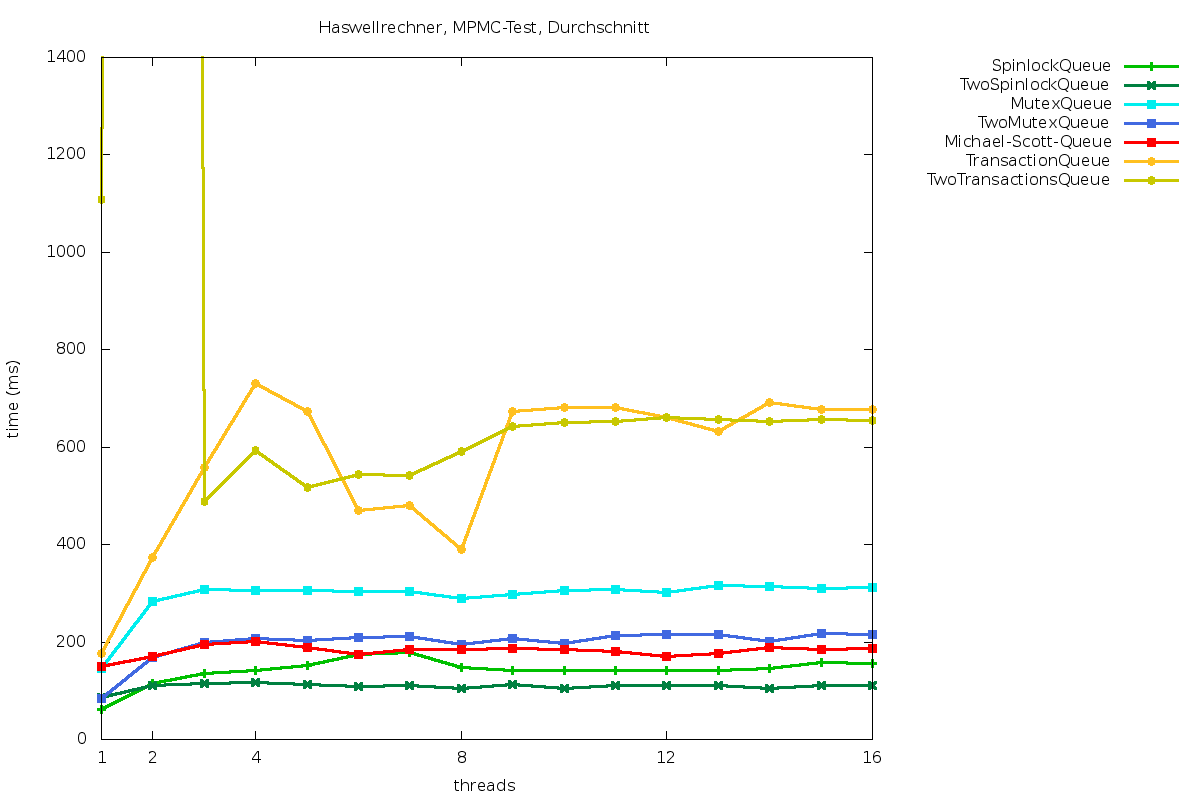
\includegraphics[width=\textwidth]{fastboxma.png}
     \end{center}
\end {figure}
\end{frame}
%-----------------------------------------

\begin{frame}
\frametitle{Ergebnisse}
\begin {figure}
      \begin{center}
	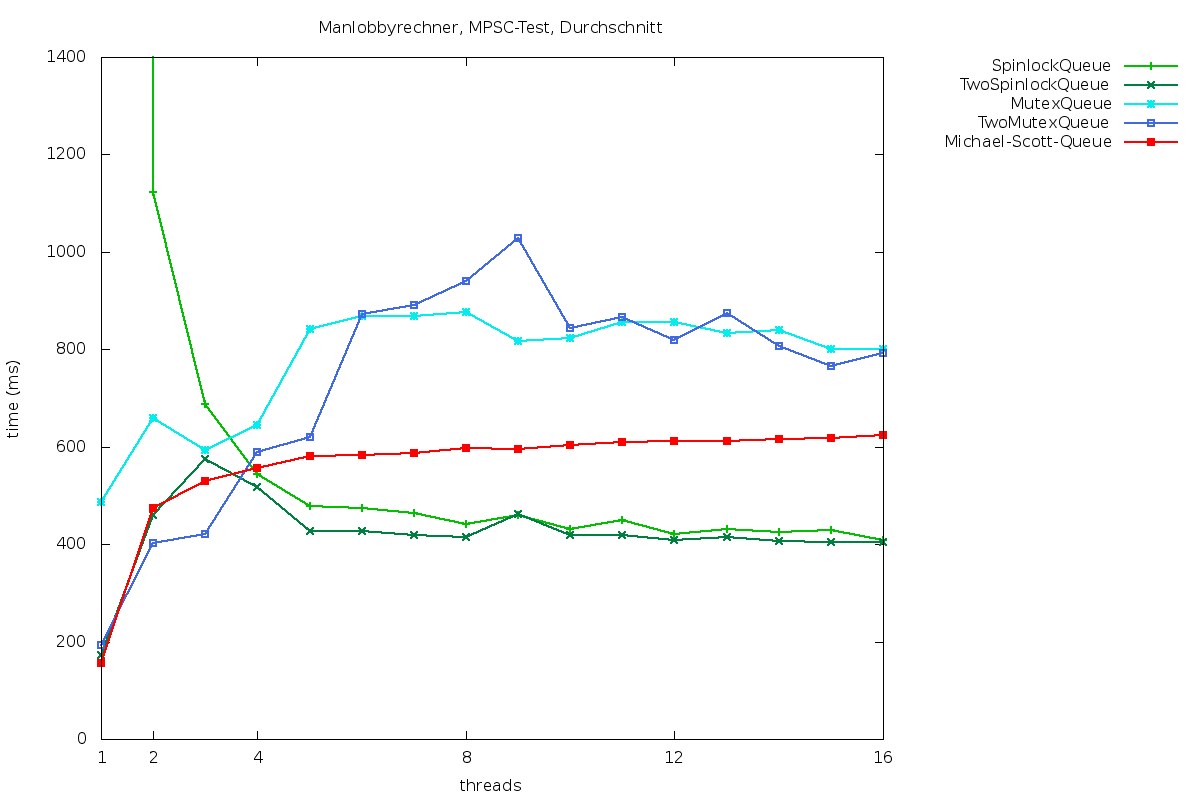
\includegraphics[width=\textwidth]{mansa.png}
     \end{center}
\end {figure}
\end{frame}

%-----------------------------------------
\begin{frame}
\frametitle{Ergebnisse}
\begin {figure}
      \begin{center}
	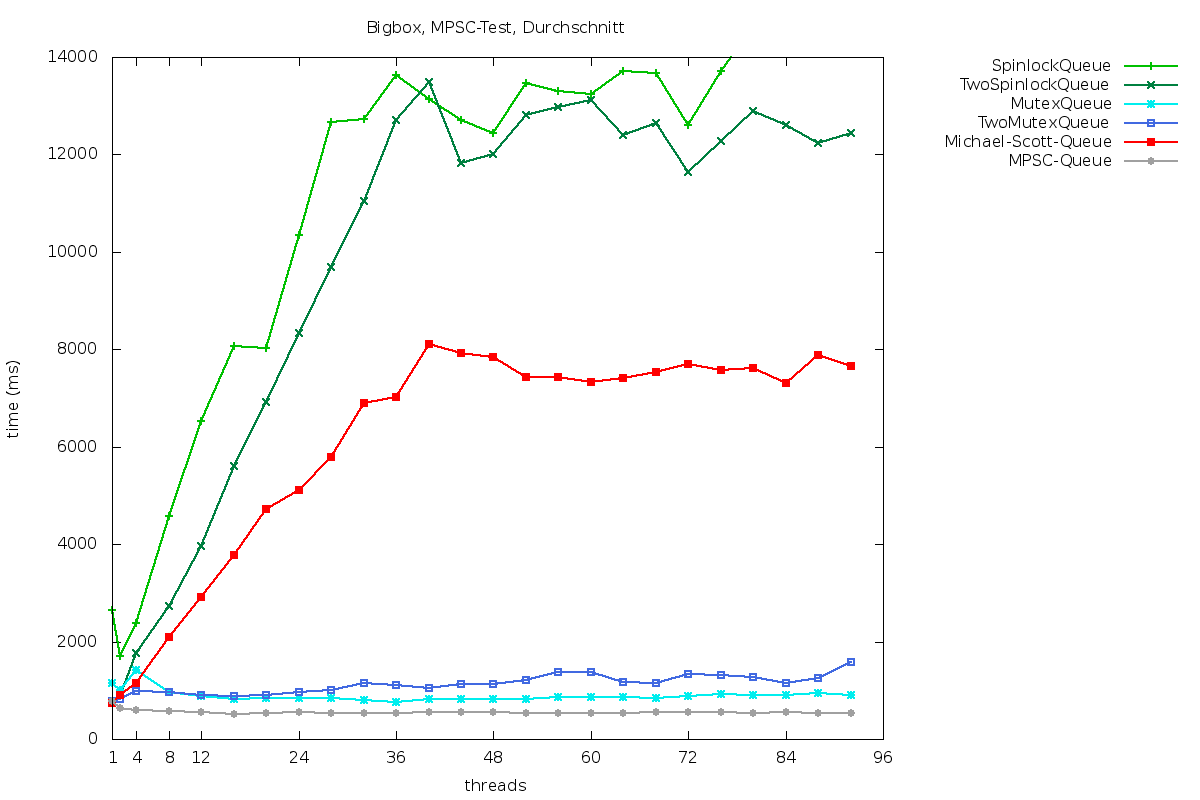
\includegraphics[width=\textwidth]{bigboxsa.png}
     \end{center}
\end {figure}
\end{frame}

%-----------------------------------------
\begin{frame}
\frametitle{Ergebnisse}
\begin {figure}
      \begin{center}
	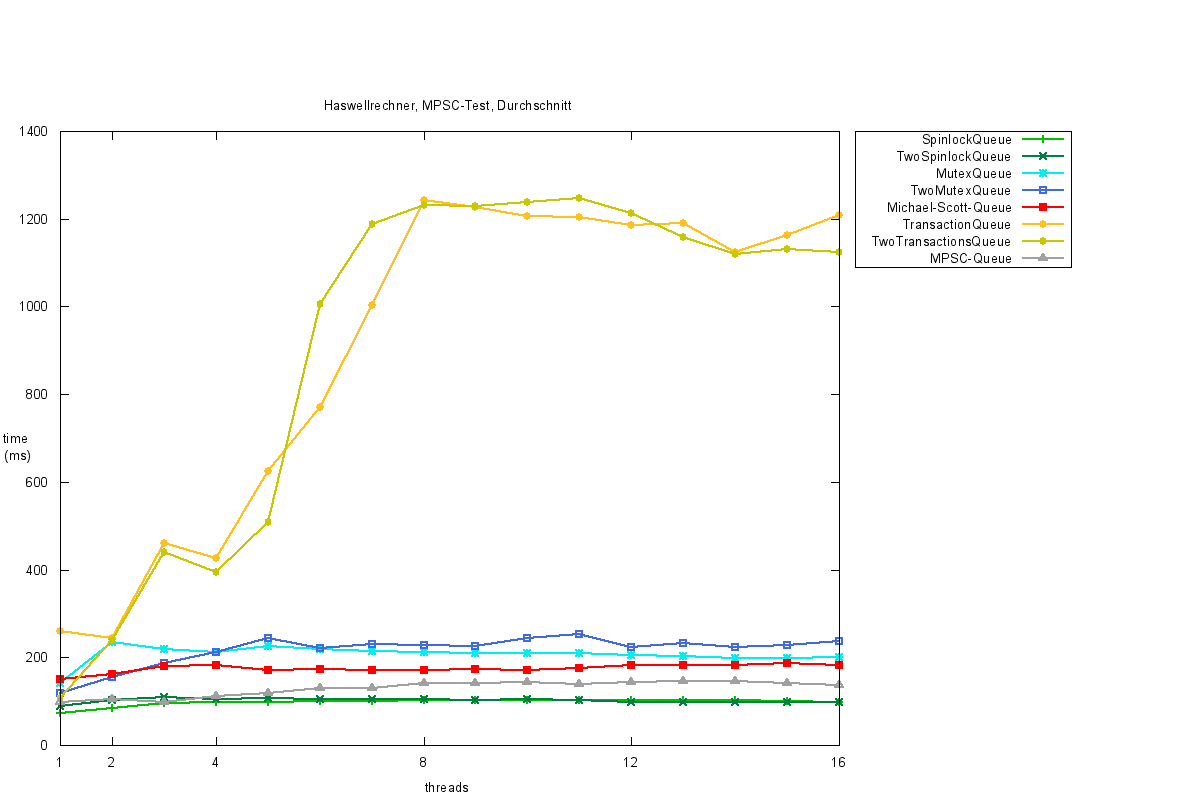
\includegraphics[width=\textwidth]{fastboxsa.png}
     \end{center}
\end {figure}
\end{frame}


%-----------------------------------------

\begin{frame}
\frametitle{Fazit}
\begin{itemize}
\item Michael-Scott Queue ist durchgehend suboptimal.\\
	Allerdings gibt es auch immer schlechtere Varianten.\\
	Insgesamt ist sie damit in jeder Hinsicht mittelm\"a\ss{}ig.
\item MPSC-Queue ist auf den meisten Systemen besser als blockierende Queues,
	aber auf Haswell Architektur wird sie von der Spinlock Queue \"uberholt.
\item Insgesamt ist es nicht offensichtlich, welche Queue unter welchen Bedingungen optimal arbeitet.
\item Messdaten, Testumgebung und verwendete Queues auf:\\
	git://github.com/Lorenz-badgers/qtpie \\
	https://github.com/Lorenz-badgers/qtpie.git
\end{itemize}
\end{frame}


%-----------------------------------------
\begin{frame}
\frametitle{Erfahrungen}
\begin{itemize}
\item nachtr\"agliche Implementierung gemeinsamer Schnittstelle zwischen verschiedenen Queues und Testsystem komplexer als erwartet
\item Messungen f\"ur pr\"asentierte Graphen sp\"ater als geplant durchf\"uhrbar
\item Umgang mit Messdaten: mehr Daten speichern, um z.B. Streuungen ermitteln zu k\"onnen
\end{itemize}
\end{frame}


%-----------------------------------------

%------------------------------------------------
\begin{frame}
\Large{\centerline{Vielen Dank f\"ur Ihre Aufmerksamkeit!}}
\end{frame}



\end{document}
